\documentclass{article}
\usepackage[T1]{fontenc}
\usepackage{lmodern}
\usepackage{graphicx}
\usepackage{amsmath,amssymb}
\usepackage[a4paper,margin=2cm]{geometry}
\usepackage[absolute,overlay]{textpos}
\setlength{\TPHorizModule}{1mm}
\setlength{\TPVertModule}{1mm}
\usepackage[indonesian]{babel}
\usepackage{hyperref}
\setlength{\emergencystretch}{2em}
% unit: Halaman 95

\begin{document}

% === Halaman 95 (llm) ===

\section*{D. Hill Cipher}

\begin{itemize}
    \item Dikembangkan oleh Lester Hill (1929), termasuk ke dalam polygram cipher yang berbasis aljabar linier
    \item Menggunakan $m$ buah persamaan linier
    \item Untuk $m = 3$ (enkripsi setiap 3 huruf), sistem persamaan linernya menjadi:
\end{itemize}

\vspace{10mm}

\begin{align*}
C_1 &= (k_{11} p_1 + k_{12} p_2 + k_{13} p_3) \pmod{26} \\
C_2 &= (k_{21} p_1 + k_{22} p_2 + k_{23} p_3) \pmod{26} \\
C_3 &= (k_{31} p_1 + k_{32} p_2 + k_{33} p_3) \pmod{26}
\end{align*}

\vspace{10mm}

\[ \mathbf{C} = \mathbf{KP} \]

% deskripsi: Representasi matriks dari sistem persamaan linier Hill Cipher untuk m=3
% bbox normalisasi: [0.5140, 0.5420, 0.9300, 0.7830]
\begin{textblock*}{87.36mm}(107.94mm,160.97mm)
\noindent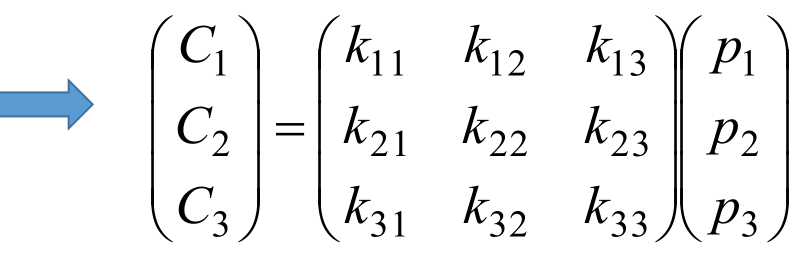
\includegraphics[width=87.36mm,height=71.58mm]{../../images/llm/page_095_img_01.png}%
\end{textblock*}

\end{document}
